
\documentclass[sigconf]{acmart}

\usepackage{graphicx}
\usepackage{booktabs}
\usepackage{hyperref}
\usepackage{subcaption}
\usepackage{listings}

\title{A Proxy Tool for Preserving and Inspecting Online Ads in Web Archives}

\author{Christopher Rauch}
\affiliation{%
  \institution{Drexel University}
  \country{USA}
}
\email{cr625@drexel.edu}

\begin{abstract}
Online advertisements are an ephemeral yet influential form of digital content. Despite their centrality to the modern web, ads are often missing or misrepresented in web archives. This demo presents an interactive proxy tool designed to capture, inspect, and preserve online advertisements in real-time browsing sessions. The system offers researchers and archivists a method to analyze the behaviors and presence of ads during web interactions. We describe the design and implementation of the tool, its use...
\end{abstract}

\keywords{web archiving, advertisements, proxy server, personalization, reproducibility}

\begin{document}

\maketitle

\begin{teaserfigure}
  \centering
  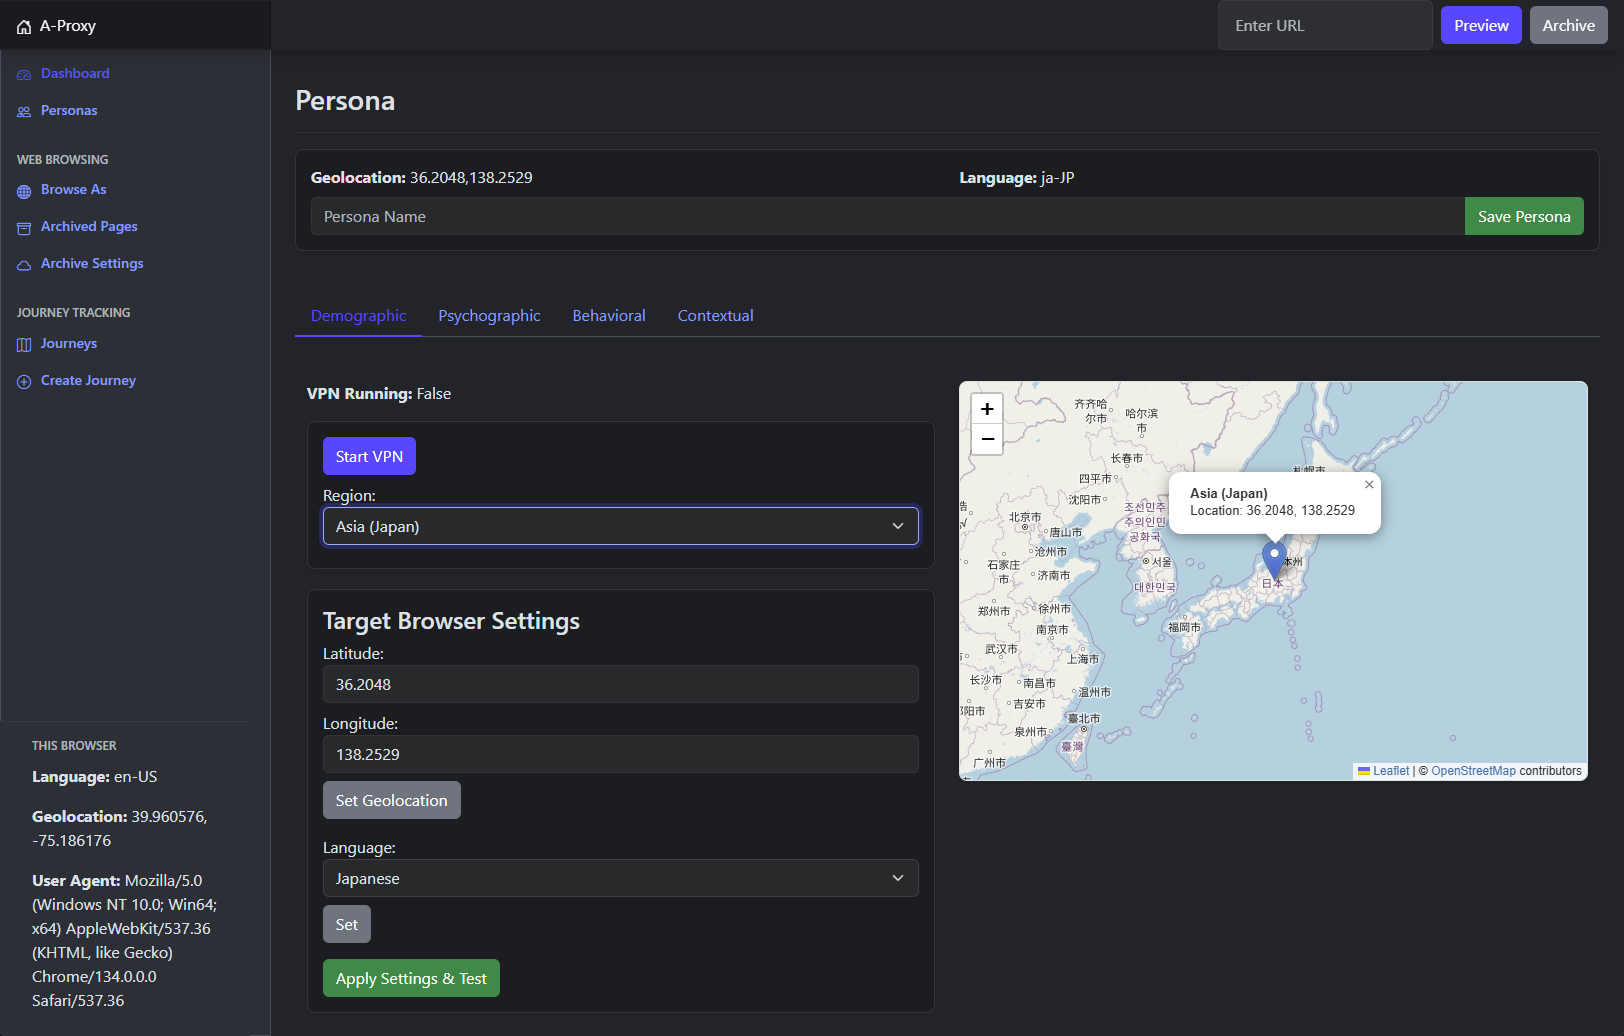
\includegraphics[width=\textwidth]{persona-teaser.png}
  \caption{Interface of the proxy system showing persona-level customization, including geolocation, language, and behavioral settings. The system enables fine-grained control over browser characteristics to simulate user experiences during web archiving or ad tracking.}
  \Description{Screenshot of A-Proxy interface showing persona settings, VPN toggle, and browser controls including geolocation and language.}
  \label{fig:persona}
\end{teaserfigure}

\section{Introduction}
Web advertisements are tailored content that play a critical role in shaping user experience, influencing opinion, and driving revenue. Despite their significance, such ads are often excluded from archived web pages due to technical and policy challenges. This gap hinders research on online influence, personalization, and ad ecosystems. To address this, we present a proxy-based tool that captures web ads as users encounter them, enabling deeper inspection and archival quality assessment.

\section{System Overview}
Our system is built as a local HTTP proxy that intercepts and logs ad-related requests during a browsing session. Users direct their browser traffic through the proxy, which records third-party requests, DOM changes, and visual captures of ad content.

\section{Use Cases}
This tool is suited for digital preservationists, researchers conducting web-based content audits, and scholars studying online influence. For example, one can use the proxy to inspect how ad content differs across user personas or to compare live versus archived versions of the same page.

\section{Implementation}
The proxy is written in Python and leverages \texttt{mitmproxy} for traffic interception and modification. Captured ad content is rendered and stored locally in a structured format. The system integrates with headless browsers to automate browsing sessions for reproducibility.

The source code is available at: \url{https://github.com/savingads/a-proxy}

A demonstration video is accessible at: \url{[INSERT VIDEO LINK HERE]}

\section{Conclusion and Future Work}
This tool aims to improve the completeness and interpretability of web archives by focusing on the visibility and behavior of online ads. Future work includes support for mobile traffic, real-time annotation, and integration with archival platforms.

\bibliographystyle{ACM-Reference-Format}
\bibliography{software}

\end{document}
